% beta
\subsection{Гамильтоновы графы}
\textbf{Гамильтоновым путём} называется простой путь, приходящий через каждую вершину графа ровно один раз.

Простой цикл, содержащий все вершины графа, называется \textbf{гамильтоновым}.

Граф называется \textbf{полугамильтоновым}, если он содержит гамильтонов путь.

Граф называется \textbf{гамильтоновым}, если в~нём есть гамильтонов цикл.

\begin{figure}[h!]
	\begin{center}
		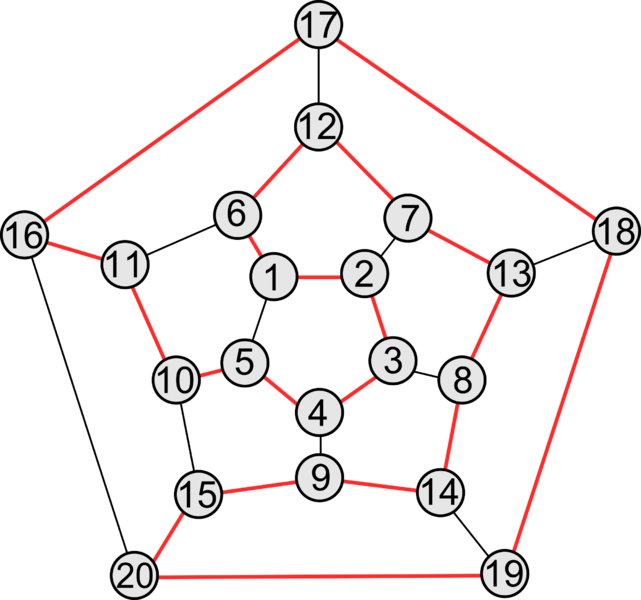
\includegraphics[scale=1.5]{./mh/discrete_mathematics/graph/EH/hamiltonian_graphs/641px-Hamiltonial.png}
	\end{center}
	\caption{Граф додекаэдра с выделенным циклом Гамильтона}
\end{figure}

\begin{theorem}[Дирака]
\label{th:Dirac}
Если в~графе~$G = (V, E)$ с~$n \geqslant 3$~вершинами $\forall u \in V \ \deg u \geqslant \frac{n}2$, то граф гамильтонов.
\end{theorem}
\begin{proof}
\begin{enumerate}
	\item Докажем методом от~противного, что граф связный.
	Пусть он несвязный.
	Выберем компоненту связности~$G' = (V', E')$ с~наименьшим числом вершин, тогда $|V'| \leqslant \frac{n}2$.
	Возьмём $v \in V'$, тогда $\deg v \leqslant |V'| - 1 < \frac{n}2$.
	Противоречие с~условием.
	\item Выберем цепь~$C = (v_0; e_0; v_1; \ldots; e_{k-1}; v_k)$ максимальной длины.
	Тогда все вершины, соседние с~$v_0$, лежат в~этой цепи, иначе можно увеличить длину цепи.
	Среди $v_1, v_2, \ldots, v_k$ не~менее $\frac{n}2$~вершин, соседних с~$v_0$, т.\,к. $\deg v_0 \geqslant \frac{n}2$.
	Аналогично для~$v_k$.
	Так же, так как цепь наибольшая, то $v_k$ либо совпадает с $v_0$, либо они не смежны.
	
	По \hyperlink{pigeonhole_principle}{принципу Дирихле} найдутся $v_{i-1}$ и~$v_i$ такие, что $v_{i-1}$ соседняя с~$v_k$, а $v_i$~--- с~$v_0$.
	
	Докажем, что $(v_i; e_{i+1}; \ldots; v_k; e; v_{i-1}; e_{i-1}; \ldots; v_0; e'; v_i)$~--- гамильтонов цикл, методом от~противного.
	Предположим обратное, тогда есть вершина~$u$, не~входящая в~цикл, и~существует $(v_0, u)$\nobreakdash-\hspace{0pt}маршрут.
	Значит, существует ребро, инцидентное одной из~вершин цикла, но не~входящее в~него, и~можно получить более длинную цепь.
	Противоречие.
\end{enumerate}
\end{proof}
\begin{proof}
Так же существует доказательство теоремы Дирака через теорему Оре.
Возьмем любые неравные вершины $u, v \in G$. Тогда $\deg u + \deg v \geqslant \frac n 2 + \frac n 2 = n$. По теореме Оре $G$ — гамильтонов граф.
\end{proof}

\begin{theorem}[Оре]
	Если в~графе с~$n \geqslant 3$~вершинами для~любых двух несмежных вершин $u$ и~$v$ $deg u + deg v \geqslant n$, то граф гамильтонов.
\end{theorem}
\begin{proof}
\begin{enumerate}
	\item Докажем методом от~противного, что граф связный.
	Пусть он несвязный, тогда в~нём найдутся хотя~бы две компоненты связности $G_1(V_1, E_1)$ и~$G_2(V_2, E_2)$.
	Пусть $u \in V_1$, $v \in V_2$. $u$ и~$v$ несмежные, тогда
	\begin{equation*}
	\deg u \leqslant |V_1| - 1, \ \deg v \leqslant |V_2| - 1 \opbr\Rightarrow \deg u + \deg v opbr\leqslant |V_1| + |V_2| - 2 \opbr\leqslant n - 2
	\end{equation*}
	
	Противоречие с~условием.
	
	\item Докажем, что граф гамильтонов.
	Выберем цепь~$W = (v_0; e_0; v_1; \ldots; e_{k-1}; v_k)$ наибольшей длины.
	В~ней содержатся все вершины, соседние с~$v_0$ или~с~$v_k$.
	Т.\,о., среди вершин $v_1, \ldots, v_k$ $deg v_0$ соседних с~$v_0$.
	Аналогично для~$v_k$.
	
	$\deg v_0 + \deg v_k \geqslant n$, тогда найдутся $v_i$ и~$v_{i+1}$ такие, что $v_i$ соседняя с~$v_k$, а $v_{i+1}$~--- с~$v_0$.\newline
	$(v_{i+1}; e_{i+1}; \ldots; v_k; e; v_i; e_{i-1}; v_{i-1}; \ldots; e_0; v_0; e'; v_{i+1})$~--- гамильтонов цикл (доказательство аналогично доказательству в теореме \ref{th:Dirac} (Дирака)).
\end{enumerate}
\end{proof}